\documentclass{VUMIFPSbakalaurinis}
\usepackage{algorithmicx}
\usepackage{algorithm}
\usepackage{algpseudocode}
\usepackage{amsfonts}
\usepackage{amsmath}
\usepackage{bm}
\usepackage{caption}
\usepackage{color}
\usepackage{float}
\usepackage{graphicx}
\usepackage{listings}
\usepackage{subfig}
\usepackage{wrapfig}

\usepackage{color}
\definecolor{todo-background-color}{rgb}{0.7, 0.7, 0.7}
\newcommand{\TODO}[1]{
\colorbox{todo-background-color}{TODO: #1}
}


% Titulinio aprašas
\university{Vilniaus universitetas}
\faculty{Matematikos ir informatikos fakultetas}
\department{Programų sistemų katedra}
\papertype{Bakalauro baigiamasis darbas}
\title{Duomenų dimensiškumo mažinimas ir klasifikavimas}
\titleineng{Dimensionality reduction and classification}
\author{Donatas Kučinskas}
\supervisor{Vytautas Valaitis}
\reviewer{Julija Vysockytė}
\date{Vilnius – \the\year}

% Nustatymai
% \setmainfont{Palemonas}   % Pakeisti teksto šriftą į Palemonas (turi būti įdiegtas sistemoje)
\bibliography{bibliografija}

\begin{document}

\maketitle

\setcounter{page}{2}
%% Padėkų skyrius
% \sectionnonumnocontent{}
% \vspace{7cm}
% \begin{center}
%     Padėkos asmenims ir/ar organizacijoms
% \end{center}

\sectionnonumnocontent{Santrauka}
Glaustai aprašomas darbo turinys: pristatoma nagrinėta problema ir padarytos
išvados. Santraukos apimtis ne didesnė nei 0,5 puslapio. Santraukų gale
nurodomi darbo raktiniai žodžiai. 
% Nurodomi iki 5 svarbiausių temos raktinių žodžių (terminų).
% Vienas terminas gali susidėti iš kelių žodžių.
\raktiniaizodziai{raktinis žodis 1, raktinis žodis 2, raktinis žodis 3, raktinis žodis 4, raktinis žodis 5}   

\sectionnonumnocontent{Summary}
Santrauka anglų kalba. Santraukos apimtis ne didesnė nei 0,5 puslapio.
\keywords{keyword 1, keyword 2, keyword 3, keyword 4, keyword 5}

\tableofcontents

\sectionnonum{Įvadas}
Klasifikavimas - tai dažnai sutinkama užduotis, turintį įvairių sprendimo būdų.
Šios uždavinio tikslas - identifikuoti, kuriai grupei priklauso tiriamas objektas.
Tiriamieji objektai dažniausiai būna vienos rūšies, aprašomi tam tikrais parametrais, o grupės, kuriems jie yra priskiriami - iš anksto žinomos.
Pavyzdžiui, galima klasifikuoti gyvūnus pagal tam tikras jų fizines savybes - kojų ilgį, storį, kitas kūno apimtis, kailio ilgį ir pan.
Natūralu, kad kiekvienas net ir tos pačios rūšies gyvūnas turės šiek tiek kitokius parametrus, tačiau šie parametrai dažniausiai turi įvairius dėsningumus, pagal kuriuos galima bandyti atspėti, kuriai rūšiai tam tikras gyvūnas priklauso.


Norint išspręsti konkretų klasifikavimo uždavinį, akivaizdžiausias sprendimas galėtų būti šių grupių parametrų ištyrimas - pavyzdžiui, norint mokėti atskirti triušius nuo liūtų turint jų ūgius nėra sunki užduotis.
Tačiau problema kyla, kai atskiriamos klasės yra labai panašios viena į kitą - tokiu atveju pastebėti tam tikrus dėsningumus ir juos sumodeliuoti bei realizuoti ir kur kas sunkiau.
Be to, sprendžiant konkretų klasifikavimo uždavinį, tektų gilintis į klasifikuojamus objektus - pavyzdžiui, norint sukurti tam tikrų kiškių rūšių klasifikavimą, gilios žinios apie šias kiškių rūšių savybes būtų privalomos.
Dažniausiai įvairūs dėsningumai apima ne vieną dydį, bet jų kombinaciją, kurią atrasti ir apskaičiuoti reikalautų daug pastangų.
O norint efektyviai atskirti tam tikras objektų klases, gali prireikti daugybės skirtingų dėsningumų.
Šios priežastys labai apsunkina efektyvaus klasifikavimo algoritmo kūrimą analizuojant klases, todėl yra retai naudojamas.

Vienas populiariausių klasifikavimo sprendimo metodų - klasifikavimas naudojant neuroninį tinklą.
Turint pakankamai didelį tiriamų objektų duomenų kiekį, galima įžvelgti tam tikrus dėsningumus.
Neuroninis tinklas leidžia tai automatizuoti - vietoje to, kad žmogus mokytųsi apie objekto savybes, tai atliekama su neuroniniu tinklu.
Turimi duomenys panaudojami apmokyti neuroninį tinklą, kuris po to geba pats pasakyti, kuriai grupei tiriamas objektas priklauso.
Žinoma, neuroninis tinklas nėra visada teisus, kadangi jis remiasi patirtimi, kurią įgijo pavyzdinių duomenų apmokymo metu, tačiau jei šie apmokymui buvo surinkta pakankamai korektiškų duomenų, neuroninis tinklas geba klasifikuoti objektus pakankamai tiksliai.

Dimensiškumo mažinimas (angl.~\textit{dimensionality reduction})
Savybių ištraukimas (angl.~\textit{feature extraction})

\TODO{TODO: pridėti paaiškinimą, kad dažniausiai turime daug duomenų?}

\TODO{neuroniniai tinklai?}
\TODO{dimensiškumo mažinimas}
\TODO{tyrimo tikslai?}

\section{Dirbtinių neuronų tinklas}

Dirbtinis neuronų tinklas - tai tarpusavyje susijungusių dirbtinių neuronų tinklas, kurio užduotis yra spręsti tam tikrą užduotį arba užduotis.
Dirbtinis neuronų tinklas gavęs pradinius užduoties duomenis, juos apdoroja ir taip gaunamas tam tikras atsakymas.
Šis atsakymas nebūtinai yra teisingas - neuronų tinklai suprojektuoti taip, kad galėtų būti mokomi kai gauna neteisingą atsakymą.

\subsection{Dirbtinis neuronas}

Dirbinių neuronų tinklas sudarytas iš daugybės dirbtinių neuronų, todėl norint suprasti tinklą, reikia pradėti nuo vieno dirbtinio neurono.
Žmogaus smegenys sudarytos iš daugybės neuronų.
Dirbtinis neuronas - tai supaprastintas šių biologinių neuronų modelis.
Jo modelis pavaizduotas \ref{fig:neuron}~paveiksliuke.
Dirbtinio neurono veikimo principas gan paprastas - per kairėje esančias jungtis dirbtinis neuronas gauna signalus iš kitų dirbtinių neuronų - iš $k$-tosios jungties gaunamas $x_k$ dydžio signalas.
Šiuos signalus neuronas apjungia ir pertvarko, ir taip sugeneruojamas dirbtinio neurono išeinamasis signalas.
Šis išeinamasis signalas gali būti siunčiamas daugybei kitų neuronų - dešinėje esančios jungtys yra neurono išeinamojo signalo jungtys, kuriomis ir yra siunčiamas išeinamasis signalas.

Dirbtinis neuronas generuoja išeinamąjį signalą pagal tam tikrą modelį.
Pirmiausia, kiekviena įeinančioji jungtis $k$ turi savo svorį $w_k$ - šis svoris yra padauginamas iš įeinančio signalo dydžio $x_k$.
Tada visos šios signalų dydžių ir svorių sandaugos yra susumuojamos - taip gaunamas skaičius $a$ (\ref{eq:a}~formulė).
Tada šis skaičius $a$ yra paduodamas kaip argumentas tam tikrai funkcijai $f$ ir gaunamas neurono išeities signalas $y = f(a)$.
Šį funkcija $f$ yra vadinama aktyvacijos funkcija - ją galima keisti pagal tai, kokio tikslo siekiama iš šio dirbtinio neurono.
Populiariausios aktyvacijos funkcijos - slenkstinė, tiesinė, hiperbolinis tangentas bei sigmoidinė (\ref{eq:sigmoid}~formulė).
Iš esmės akvyvacijos funkcija gali būti bet kokia funkcija, tačiau vėliau norint apmokyti dirbtinį neuronų tinklą, reikia rasti šios funkcijos išvestinę.
Dėl šios priežasties dažniausiai pasirenkamos tokios aktyvacijos funkcijos, kurios ne tik tinkamai pertvarko signalą išvedimui, tačiau ir kurios išvestinės yra paprastos.

Įeinamosios neurono jungtys numeruojamos nuo 1 iki $k$.
Norint $a$ reikšmę padaryti tinkamesnę neuroninio tinklo funkcijoms, dažniausiai įvedama papildoma $0$-inė jungtis su svoriu $w_0$ ir signalo stiprumu $x_0 = 1$.
Tokiu būdu prie $a$ (formulė~\ref{eq:a}) reikšmės papildomai pridedama $w_0 * x_0 = w_0$ reikšmė.



\begin{figure}
	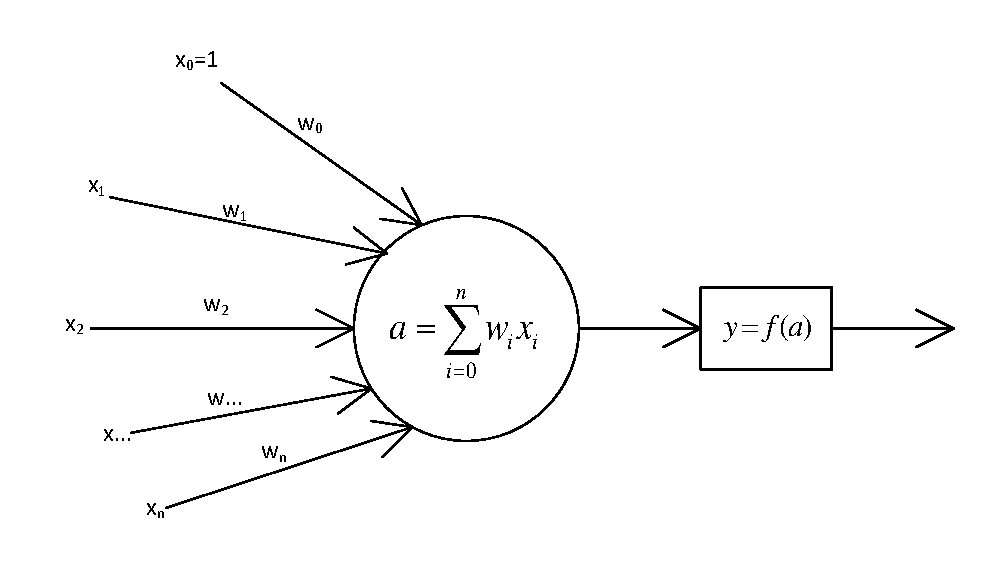
\includegraphics[scale=0.75]{diagrams/1_neuron}
	\caption{Dirbtinis neuronas}
	\label{fig:neuron}
\end{figure}

\begin{equation} \label{eq:a}
a = \sum_{k=1}^N w_kx_k
\end{equation}

\begin{equation} \label{eq:sigmoid}
f(a) = \frac{1}{1 + e^{-a}}
\end{equation}



\subsection{Dirbtiniai neuronai/tinklas?}

\TODO{finish}

Dirbtinių neuronų tinklas (angl.~\textit{Artificial neural network}) - tai tinklas, kurį sudaro dirbtiniai neuronai bei jungtys, jungiančios kai kuriuos dirbtinius neuronus.
Per kiekvieną jungtį gali eiti signalas, kuris perduoda vieno neurono išeinamąjį signalą kitam neuronui.
Kiekvienas neuronas gali turėti bet kokį skaičių įeinančių ir bet kokį skaičių išeinančių jungčių.

Kai kurios jungtys gali būti prijungtos tik prie vieno neurono.
Jungtys, kurios įeina į neuroną tačiau neišeina iš jokio neurono, naudojamos duomenų perdavimui - šiomis jungtimis neuronų tinklui perduodami signalai, atitinkantys duomenis.
Jungtys, išeinančios iš neurono tačiau neįeinančios į jokį neuroną, naudojamos rezultato gavimui - kai per visą neuroninį tinklą pereina signalai, būtent šiose jungtyse ir yra gaunamas pateiktus duomenis atitinkantis atsakymas.

Dirbtinio neuronų tinklo užduotis - pagal pateikiamus duomenis sugeneruoti atsakymą.
Pirmiausia duomenys pateikiami per tam skirtas jungtis.
Neuronai, prijungti prie šių jungčių, gauna šiuos pradinius signalus, juos apdoroja ir pradeda skleisti tam tikro stiprumo signalą išeinančiomis jungtimis.
Taip signalai sklinda tolyn ir visi tinklo neuronai būna apdorojami tol, kol galiausiai rezultatas būna gaunamas tam skirtose jungtyse.


Neuronų tinklo pateiktas atsakymas nebūtinai yra teisingas - neuronų tinklas suprojektuotas taip, kad jį būtų galima tobulinti pagal daromas klaidas.
Vienas populiariausių būdų, kuris yra naudojamas šiame darbe - atgalinė propogacija (angl.~\textit{Backpropogation}).
Tam, kad būtų galima apmokyti neuronų tinklą spręsti konkrečią problemą, reikia turėti nemažą šios problemos pavyzdinių duomenų rinkinį bei iš anksto žinoti kiekvienų duomenų teisingą atsakymą.
Mokymas vyksta pažingsniui, vienu metu neuroninui tinklui pateikiant vienus duomenis iš turimo duomenų rinkinio.
Neuroninis tinklas, gavęs duomenis, juos analizuoja ir pateikia tam tikrą atsakymą.
Šis gautas atsakymas yra sulyginamas su teisingu, iš anksto žinomu atsakymu.
Pagal tai, kaip neurininio tinklo pateiktas atsakymas skiriasi nuo teisingojo, neuroninis tinklas būna pertvarkomas.
Pertvarkymas vyksta nagrinėjant neuroninį tinklą priešinga tvarka, nei buvo nagrinėjama, kai neuroninis tinklas analizavo pateiktus duomenis.
Nagrinėjant kiekvieną neuroninio tinklo neuroną, į jį įeinančių jungčių svoriai $w_k$ (įskaitant ir $w_0$, kuris naudojamas kaip papildomas parametras) būna pakeičiami taip, kad neuroninis tinklas gautų panašesnį atsakymą į teisingąjį.

Taip atlikus vienų duomenų iš rinkinio apmokymą, imami kiti duomenys iš šio rinkinio ir mokymas kartojamas.
Kiekvienus duomenis iš šio rinkinio rekomenduotina naudoti apmokymui bent kelis kartus, kadangi neuroninis tinklas ne iš karto teisingai išmoksta spręsti problemą su konkrečiais duomenimis.
Taip pat apmokant tinklą su vienais duomenimis, neuroninio tinklo parametrai gali būti pakeisti taip, kad neuroninis tinklas nebegebės teisingai išspręsti prieš teisingai išspręstų duomenų.
Tačiau per daug mokyti neuroninį tinklą taip pat nerekomenduotina, kadangi vėliau tinklas per daug prisitaiko prie jam apmokyti naudojamo duomenų rinkinio, o ne prie problemos (angl.~\textit{Overfitting}).
Nors ir gali pasirodyti, kad neuroninio tinklo pateikiami rezultatai vis labiau ir labiau panašėja į teisingus, tačiau išbandžius šį neuroninį tinklą su kitu šios problemos duomenų rinkiniu galima įsitikinti, kad rezultatai po kurio laiko pradeda blogėti.
\TODO{įdėti (angl. Validation group)?}

\TODO{error'o skaičiavimas?}

\TODO{backpropogation?}

\subsection{Daugiasluoksnis perceptronas}

Daugiasluoksnis perceptronas - tai tam tikromis savybėmis pasižymintis dirbtinių neuronų tinklas.
Tai viena populiariausių dirbtinių neuroninių tinklų rūšis, kadangi savybės, kuriomis šis tinklas pasižymi, leidžia padaryti tam tikras skaičiavimo optimizacijas bei pakankamai lengvai realizuoti veikiantį neuroninį tinklą.
Be to, galima keisti daugiasluoksnio perceptrono parametrus pritaikant jį konkrečiai sprendžiamai problemai.

Neuronų tinklą galima nagrinėti kaip grafą, kuriame dirbtiniai neuronai yra grafo viršūnės, o jungtys, jungiančios juos - kryptinės grafo briaunos.
Jeigu neuronų tinklo grafe būtų bent vienas ciklas, tai reikštų, kad šiame cikle esančiomis jungtimis einantys signalai gali keistis ne kartą - atnaujinus tam tikro neurono išvedimo signalą, ciklu gali pakisti ir šio neurono įvedimo signalas.
Tada reikėtų vėl atnaujinti šio neurono išvedimo signalą, o tai darant vėl gali pakeisti bet kurį įvedimo signalą ir t.t.
Tai apsunkina dirbtinių neuronų veikimą, todėl dažniausiai naudojami neuronų tinklai, kuriais signalai skleidžiami pirmyn (angl.~\textit{feedforward}).
Pagal apibrėžimą, jeigu tinklo grafe nėra nei vieno ciklo, tinklas yra pirmyn skleidžiamas.

Tai, kad daugiasluoksnis perceptronas yra skleidžiamas pirmyn, suteikia nemažai privalumų.
Norint apdorojant tam tikrą neuroną, privalu žinoti visus įeinančiųjų jungčių signalų dydžius, o tai reiškia, kad jau turi būti apdoroti visi neuronai, kurių išeinamosios jungtys įeina į apdorojamąjį neuroną.
Grafe be ciklų rasti tokią seką, kuria būtų galima apdoroti tinklo neuronus nėra sunku - šį užduotis yra plačiai žinoma ir vadinama topologiniu rikiavimu.
Yra žinoma, kad beciklinį grafą visada galima topologiškai išrikiuoti, o tai reiškia, kad daugiasluoksnį perceptroną galima apdoroti tiesiog paeiliui apdorojant topologiškai išrikiuotų viršūnių seką.
Šį sąvybė palengvina neuroninio tinklo apdorojimą.

\TODO{LAYERS}

Tai reiškia, kad grafą galima išrikiuoti topologiškai, t.y. susidaryti tokią viršūnių seką, kuria galėsime apdoroti dirbtinį neuroninį tinklą.

Yra žinoma, kad 
Kadangi pirmyn skleidžiami grafai neturi ciklų,
Yra žinoma, kad kryptinį grafą, neturintį 

nėra ciklų
topologinis rikiavimas


\TODO{tam pasitarnauja topologinis rikiavimas}

\TODO{Jei būtų ciklas, reikėtų pastoviai atnaujinti.}


Visi tinklo dirbtiniai neuronai veikia pagal anksčiau aprašytą modelį - 



\TODO{dirbtinio neurono paveiksliukas}


\TODO{citata?}


\TODO{110 iš knygos}


\section{Dimensiškumo mažinimas}


Klasifikavimo problema

Galimi sprendimai:

	* statistinis sprendimas
	* neuroniniai tinklai
		* veikimas
		* apmokymas
		* validavimas?
		* Klasifikavimas požymių išskyrimui
		* Dimensiškumo mažinimas -> Klasifikavimas

\subsection{Statistinis sprendimas}

Vienas iš galimų dimensiškumo mažinimo sprendimo būdų - tiesinė diskriminantinė analizė (angl.~\textit{Linear discriminant analysis}).

\url{http://en.wikipedia.org/wiki/Linear_discriminant_analysis#Face_recognition}

\TODO{Pavyzdinio rezultato paveiksliukas}

\TODO{Minusai - tiesinė priklausomybė (evernote: idėjos)}


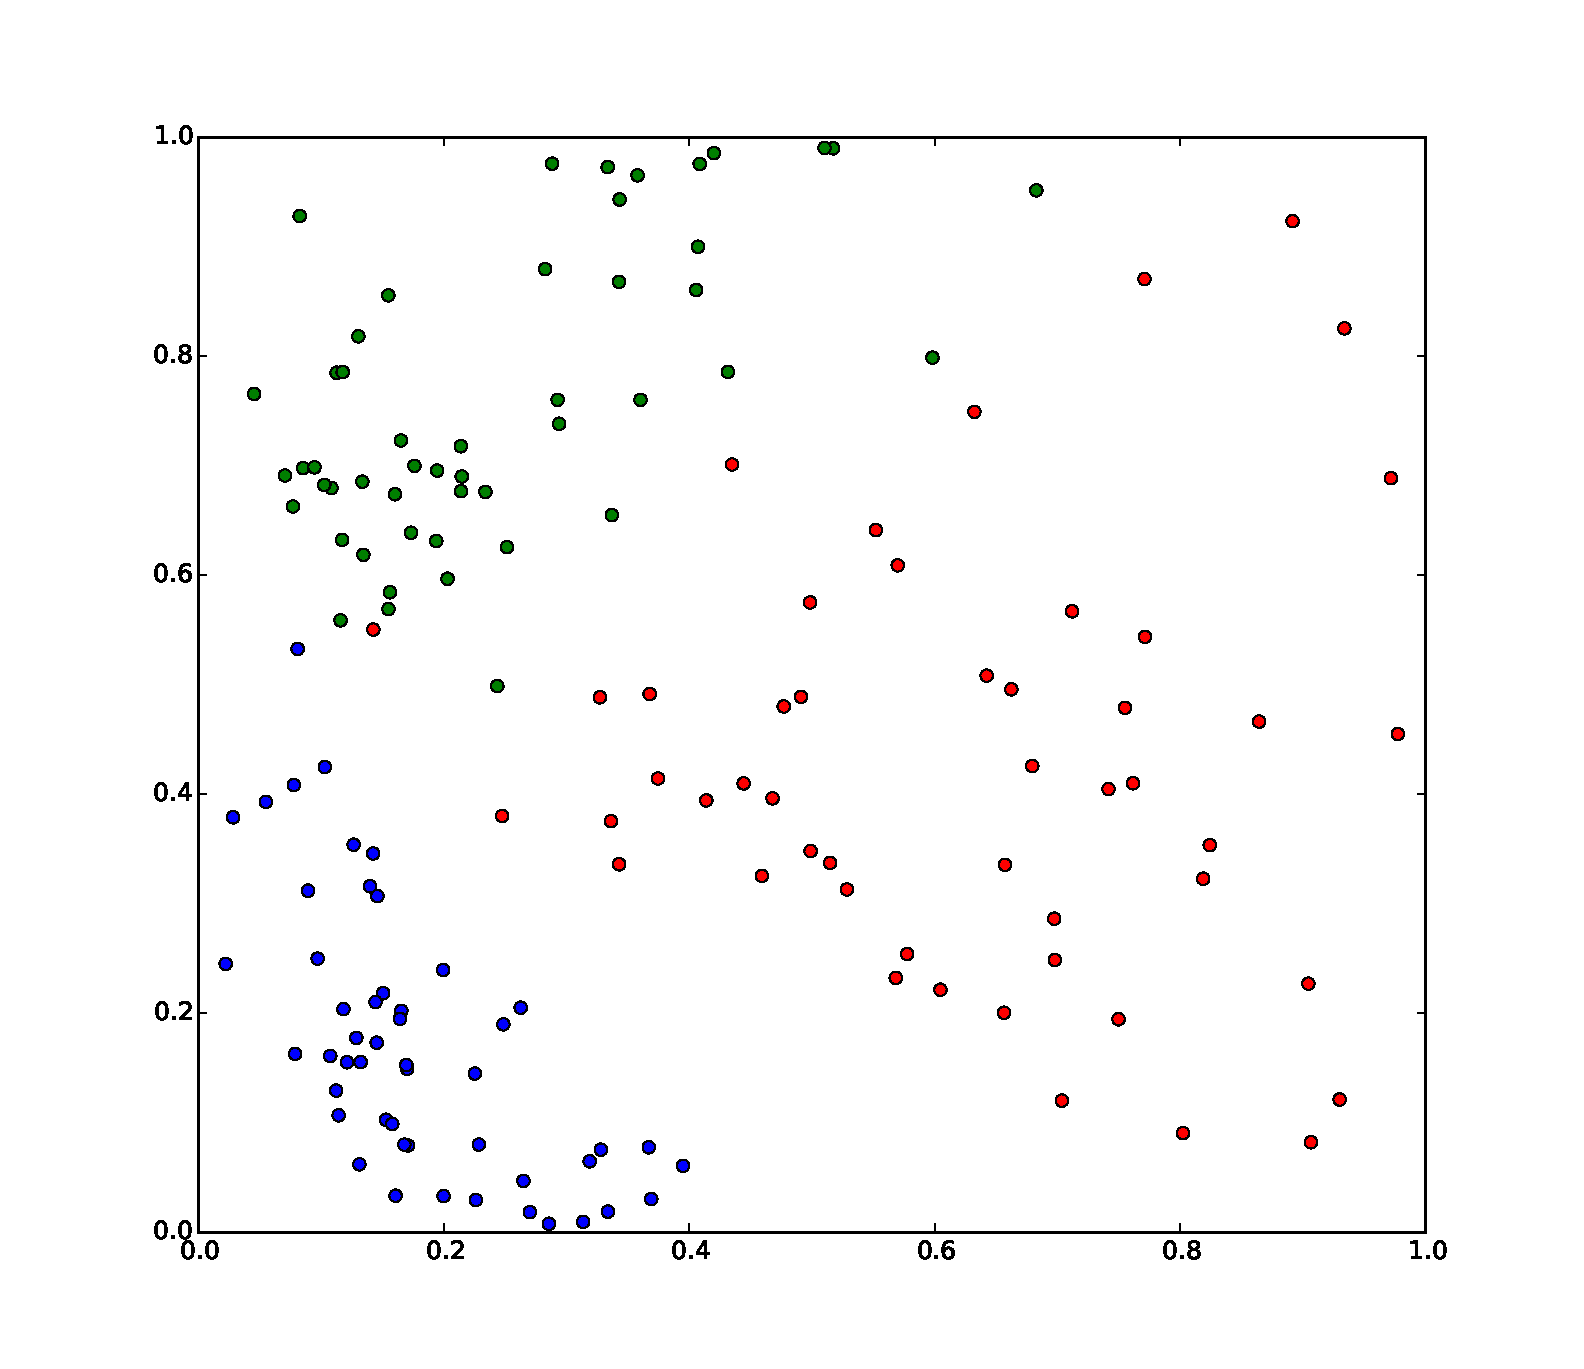
\includegraphics[width=\linewidth]{pics/classification}


\section{Vilkdagių duomenys}

Programuojant neuroninius tinklus, testavimui buvo panaudoti vilkdagių (angl.~\textit{Iris flower}) duomenys.
Tai plačiai taikomi ir viešai pasiekiami duomenys, aprašantys 3 rūšių vilkdagius.
Aprašyta po 50 kiekvienos rūšies vilkdagių.
Kiekvienas vilkdagis aprašomas pateikiant 4 dydžius: taurėlapio ilgis, taurėlapio plotis, vainiklapio ilgis bei vainiklapio plotis.
Šiuos vilkdagių duomenis sudaro 150 gėlių, kurių kiekviena aprašyta 4 parametrais bei priskirta vienai iš 3 vilkdagių grupių.

Šie duomenys puikiai tinka klasifikavimo tinklo apmokymui - tinklo tikslas yra kuo mažiau klystant pasakyti, kuriai iš 3 vilkdagių rūšių tam tikra gėlė su tam tikrais parametrais priklauso.
Be to, yra pakankamai duomenų, kad būtų galima dalį jų panaudoti tinklo apmokymui, o kitą dalį - testavimui.
Tokiu būdu bus užtikrinama, kad tinklas teisingai išmoko atskirti vilkdagių rūšis pagal parametrus, o ne tiesiog prisitaikė prie mokymui panaudotų duomenų.

\TODO{nuoroda į Vilkdagių duomenis}

\section{Genų duomenys}

\TODO{atnaujinti čia panaudotų duomenų sąvokas kitur (įrašas).}

Duomenis sudaro 12000 genų įrašų.
Kiekvienas genas aprašytas 30-čia parametrų, apibūdinančių geno savybes.
Visos parametrų reikšmės yra natūralieji skaičiai.
Kiekvienas genas priklauso vienai iš 24 grupių.
Visos genų grupės turi po 500 genų.


\section{Duomenų normavimas}

Analizuojami duomenų parametrai gali būti labai skirtingi, kadangi jie išreiškia skirtingas savybes, dydžius.
Skiriasi parametrų mąsteliai - pvz. vieno parametro reikšmės gali kisti intervale $[0; 10]$, o kito $[10^3; 10^9]$.
Dėl šių skirtumų tokias parametrų reikšmes tiesiai pateikti neuroniniui tinklui nėra praktiška.
Taip atsitinka dėl neuroninio tinklo veikimo principo - parametrai, kurių reikšmės linkusios būti didesnėmis, turėtų didesnę įtaką rezultatui nei parametrai su mažesnėmis reikšmėmis, kadangi pradiniai duomenų signalai būtų daug stipresni parametrų su didesnėmis reikšmėmis.
Tačiau daug naudingiau būtų visiems parametrams suteikti vienodą svarbą, kadangi parametro reikšmių intervalas neturi nieko bendro su parametro svarba - gali būti ir taip, kad dideles reikšmes įgyjantis parametras yra kur kas mažiau svarbus nei mažas reikšmes įgyjantysis.
Dėl šios priežasties prieš pateikiant duomenis neuroniniui tinklui, juos svarbu normuoti.

Normuojant duomenis, kiekvienas duomenų parametras normuojamas atskirai.
Norint sunormuotį parametrą, reikia išnagrinėti turimas šio parametro reikšmes bei pakeisti jas naujomis.
Sunormalizavus duomenis, visi parametrai turėtų turėti beveik lygią svarbą neuroniniui tinklui - jų reikšmių intervalai turėtų būti lygūs.
Paprasčiausias parametro normavimo metodas - rasti minimalią $p_{min}$ ir maksimalią $p_{max}$ parametro reikšmes ir kiekvieną $i$-tojo įrašo analizuojamo parametro reikšmę $p_i$ pakeisti pagal formulę:

\begin{equation}
p_i = \frac{p_i - p_{min}}{p_{max} - p_{min}}
\end{equation}

Šis metodas užtikrina, kad naujos parametro reikšmės būtų intervale $[0; 1]$.
Šis metodas buvo naudojamas tyrimo pradžioje, kadangi tai turbūt paprasčiausias ir lengvai sugalvojamas metodas.
Visgi vėliau buvo pradėtas naudoti kitas metodas - radus parametro vidurkį $p_{mean}$ ir vidutinį nuokrypį $p_{std}$, kiekviena $i$-tojo įrašo analizuojamo parametro reikšmė keičiama pagal formulę:

\begin{equation}
p_i = \frac{p_i - p_{mean}}{p_{std}}
\end{equation}

Šiuo metodu gaunamų reikšmių vidurkis lygus nuliui, o dispersija lygi vienetui.
Bandymu metu, šis metodas pasirodė tinkamesnis tiriamai problemai.

\ref{ref-gaussian}

\cite{638621}
\TODO{gauso metodo straipsnis?}

\TODO{aprašyti, kad buvo naudota iš pradžių?}
\TODO{palyginti abiejų normavimų efektyvumą?}


\TODO{ASD}

Kitas, šiame darbe naudojamas



\TODO{rezultatų palyginimas?}



\section{Dimensiškumo mažinimas neuroniniu tinklu}


\TODO{įžanga}

Dimensiškumo mažinimui taip pat buvo panaudotas neuroninis tinklas.
Turint $N$ dimensijų ir norint jas sumažinti iki $M$, kai $M < N$, tai buvo atliekama sukūrus neuroninį tiklą, kurio pirmąjame ir paskutinimae sluoksniuose yra po $N$ neuronų, o viename iš vidinių sluoksnių - $M$ (šį vidinį sluoksnį vadinkime kompresijos sluoksniu).
Tokio neuroninio tinklo užduotis nėra tiesiog sumažinti dimensijų skaičių - tai daroma netiesiogiai.
Šiam tinklui perduodant tam tikrus $M$ dimensijų turinčius duomenis, iš jo tikimasi, kad išeities neuronuose susiformuos rezultatas, lygus pradiniams duomenims - tai yra neuronų tinklas šių duomenų nepakeis.
Ši užduotis paprastai nebūtų sunki, jeigu visi vidiniai turėtų bent $N$ dimensijų - tada pateikiami duomenys galėtų būti tiesiog perkeliami iš vieno neuronų sluoksnio į kitą nepakeisti.
Tačiau kompresijos sluoksnis turi tik $M$ neuronų - vadinasi, duomenis reikės tam tikru būdu pertvarkyti, kad jie galėtų būti perduodami per šį sluoksnį prarandant kuo mažiau savybių.
Būtent čia ir įvyksta dimensiškumo mažinimas - neuroninis tinklas yra apmokomas pateikti kuo panašesnius duomenis į pradinius, ko pasekoje kompresijos sluoksnyje su $M$ neuronų yra gaunami duomenys, turintys mažiau dimensijų.
Norint sumažinti tam tikro duomens dimensijas, užtenka šį duomenį paduoti apmokytui neuroniniui tinklui ir pažiūrėti, kokie duomenys susidarė kompresijos sluoksnyje.
Nuskaičius šių neuronų reikšmes ir bus gaunamas duomuo, turintis mažiau dimensijų.

Tokiame apmokytame neuroniniame tinkle visi sluoksniai, esantys kairėje nuo kompresijos sluoksnio, yra naudojami dimensiškumo mažinimui.
Būtent per šiuos sluoksnius einant signalams ir yra sudaromas mažiau dimensijų turintis duomuo.
Kadangi šio neuroninio tinklo tikslas yra pateikti rezultatą, kuris būtų kuo panašesnis į pateiktus duomenis, todėl galima teikti, kad sluoksniai, esantys dešinėje nuo kompresijos sluoksnio, yra naudojami pradinių duomenų atstatymui.

\TODO{diagrama su dimensijų mažinimo neuroniniu tinku (kompresijos, dekompresijos pusės; N, M neuronų; rezultatas toks pat kaip duomenys)}



\sectionnonum{Rezultatai ir išvados}
Rezultatų ir išvadų dalyje išdėstomi pagrindiniai darbo rezultatai (kažkas
išanalizuota, kažkas sukurta, kažkas įdiegta), toliau pateikiamos išvados
(daromi nagrinėtų problemų sprendimo metodų palyginimai, siūlomos
rekomendacijos, akcentuojamos naujovės). Rezultatai ir išvados pateikiami
sunumeruotų (gali būti hierarchiniai) sąrašų pavidalu. Darbo rezultatai turi
atitikti darbo tikslą.

\printbibliography[heading=bibintoc]  % Šaltinių sąraše nurodoma panaudota
% literatūra, kitokie šaltiniai. Abėcėlės tvarka išdėstomi darbe panaudotų
% (cituotų, perfrazuotų ar bent paminėtų) mokslo leidinių, kitokių publikacijų
% bibliografiniai aprašai. Šaltinių sąrašas spausdinamas iš naujo puslapio.
% Aprašai pateikiami netransliteruoti. Šaltinių sąraše negali būti tokių
% šaltinių, kurie nebuvo paminėti tekste. Šaltinių sąraše rekomenduojame
% necituoti savo kursinio darbo, nes tai nėra oficialus literatūros šaltinis.
% Jei tokių nuorodų reikia, pateikti jas tekste.

% \sectionnonum{Sąvokų apibrėžimai}
\sectionnonum{Sutartinis terminų žodynas}
Sąvokų apibrėžimai ir santrumpų sąrašas sudaromas tada, kai darbo tekste
vartojami specialūs paaiškinimo reikalaujantys terminai ir rečiau sutinkamos
santrumpos.

\end{document}
